\chapter{Representing IACT data}
%
IACTs aim at reconstructing the energy, source position and particle type of
cosmic rays via their Cherenkov-light. The Cherenkov-light flashes that are
only nano seconds in duration are measured and can be separated from background
light from stars or ambient light by their brightness and topology within the
camera image. There are different ways to represent air-shower data. FACT uses
the so called largest-pulse representation (LP), whereas this work focuses on a novel
data format, both of which are described in the following chapter.

\section{The Largest-Pulse representation}
%
Data taken by an Imaging Air Cherenkov Telescope, like FACT, is usually represented in so called time series.
These time series owe their name to the fact that they represent voltages at
the photosensors over time. Within these time series lie so called large- or main-pulses
that represent the increased voltage that a charge deposition of an air-shower
causes. So, by looking for those main-pulses, shower events can be found upon
the detector noise and ambient light in the camera. Of course, the main-pulses
consist of multiple photon signals and noise superposed over time, but in this
state they are electric pulses representing the response of very specific
hardware. So rather than measuring physical properties, this means that the
charge deposit has to be interpretated to be transferred into physics
observables, independent of these specifics.
Such interpretations always include assumptions of physical and technical
kinds. By integrating the charge in one pixel an equivalent of a photon count
can be obtained, called the \textit{photon equivalent} (PE). So the first
observable in this representation is the PE which corresponds to the best
estimate of the number of photons measured per pixel. The photon counts are
spatially located by the corresponding pixel they are assigned to. The 1440
pixels of FACT are the determining grid that yield the spatial coordinates of
every shower event.

The second observable is the time. When the telescope is triggered and records
data the arrival time of the event is measured via the time information within
the time series. From the time series a quantized timing information per pixel
can be developed by dividing the event into time slices. From this the arrival
time of the photons per pixel can be calculated by averaging. Thus, the arrival
times $t$ per pixel are the second observable of the LP event
representation, besides the photon-equivalents.

\begin{figure}
  \begin{subfigure}{0.475\textwidth}
    \includegraphics[width=1.1\textwidth, page=40]{Plots/cleaning_facttools_pe_20131104_162.pdf}
  \end{subfigure}
  \begin{subfigure}{0.475\textwidth}
    \includegraphics[width=1.1\textwidth, page=40]{Plots/cleaning_facttools_arrival_times_20131104_162.pdf}
  \end{subfigure}
  \caption{The measured observables of the LP representation are shown as scatter plots within the pixels. On the left the distribution of photon-equivalents $c$ of a typical shower event (Crab observation on November, 4th 2013, run 162, event 80) is shown. On the right the arrival times of that event's photons with respect to the mean arrival time in ns are displayed.}
  \label{fig:mainpulse}
\end{figure}

\section{The PhotonStream representation}
\label{sec:phs}
%
The PhotonStream representation aims at creating a data format consisting of photons by storing their observed physical properties. This data representation, its extraction from the data and the cleaning process are based on Sebastian Mueller's work \cite{sebastian, photonstream, phs}. From the measured time series single photons are extracted instead of deriving photon counts in pixels. Each of these photons is assigned an arrival time and pixel, creating a list of arrival times per photon for each pixel. By doing so, a 3-dimensional data set is created, which can be represented in form of so called point clouds (\autoref{fig:point_cloud}).
%
\begin{figure}
  \centering
  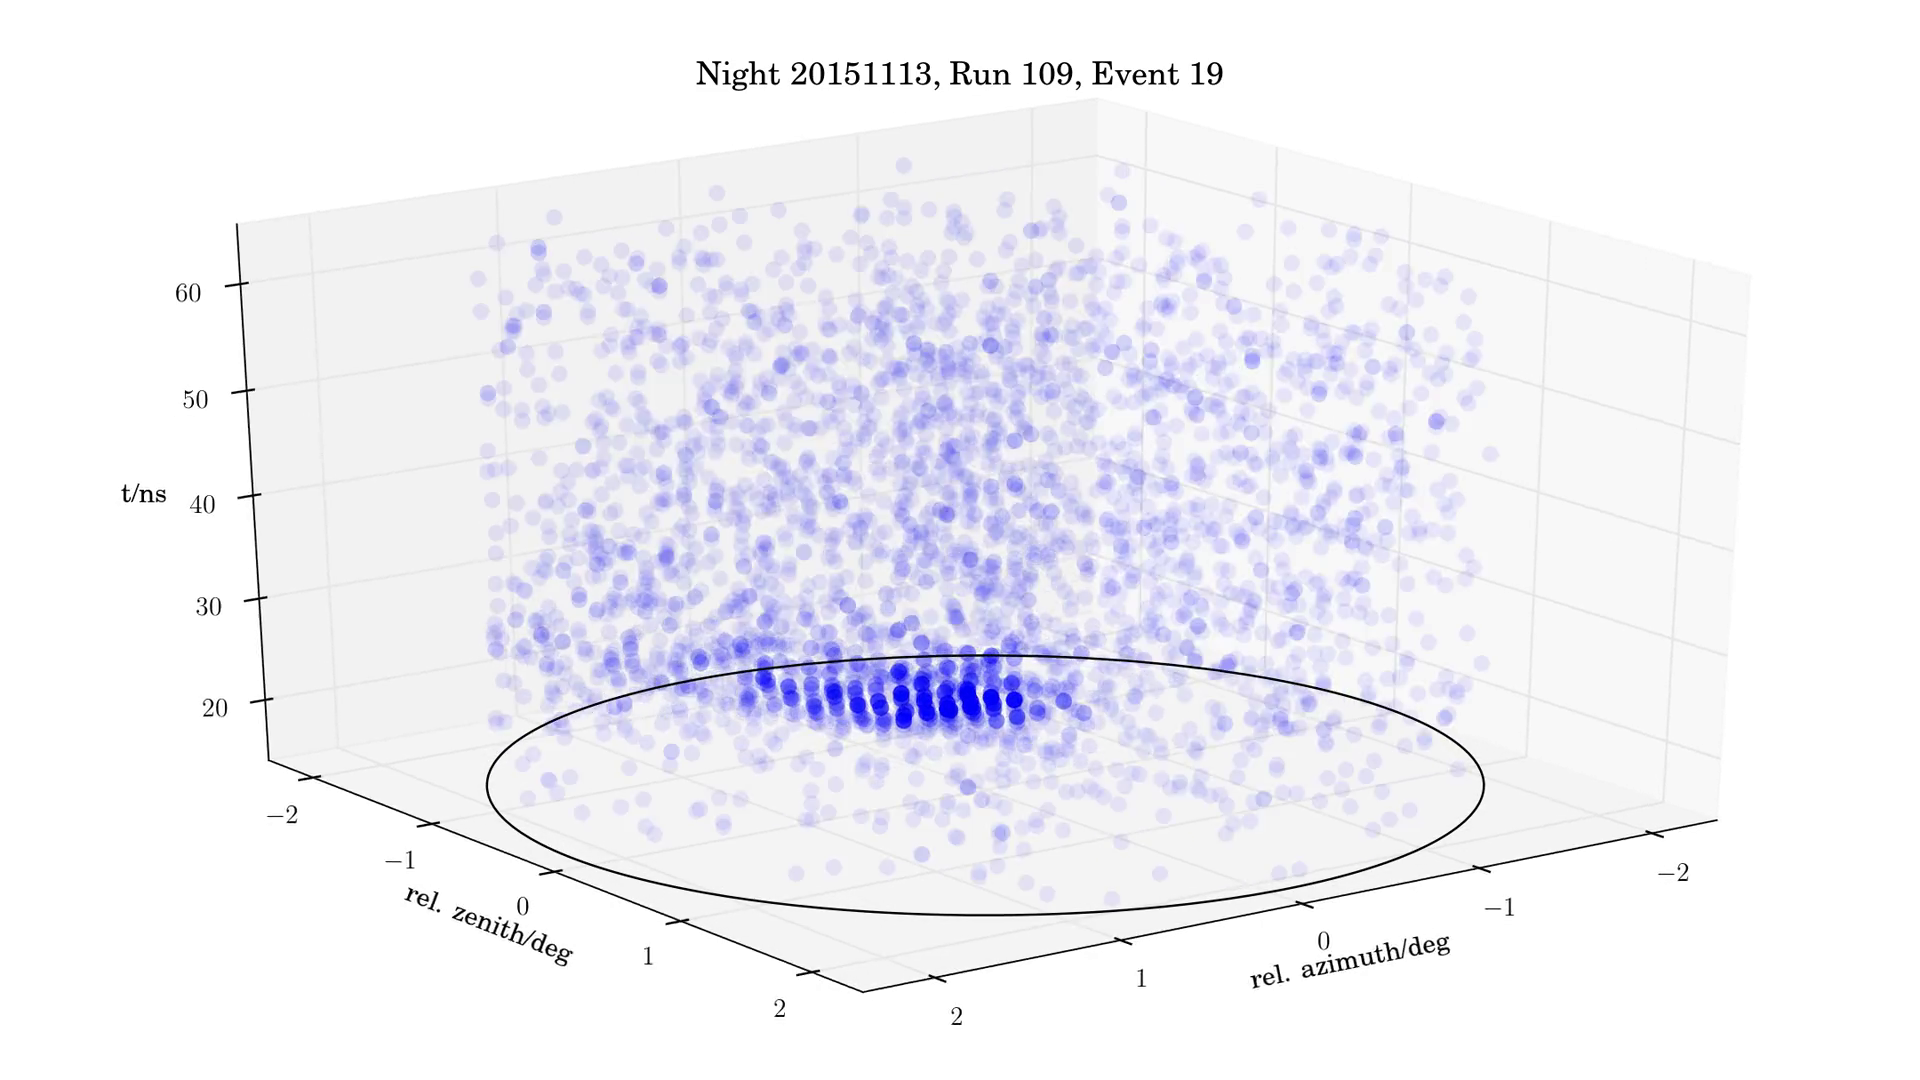
\includegraphics[width=0.95\textwidth]{Plots/event2.png}
  \caption{Uncleaned event represented by the 3-dimensional point cloud of the Photonstream. Every blue sphere represents a measured photon in the corresponding time slice and pixel.}
  \label{fig:point_cloud}
\end{figure}
%
\subsection{Single Photon Extraction}
%
To generate the PhotonStream data from the measured time series, single photons
need to be found and extracted. FACT is sampling recorded events with a
frequency of $\SI{2}{\giga\hertz}$. This yields a very high time resolution, but still quantized values within the time series. The time series consists of multiple signals
of single photons and different kinds of noise. Among the latter are several
electronic artifacts. The photon extraction does not take such artifacts into
account, so the data has to be cleaned of those at first. Unfortunately there
are rare kinds of artifacts that can not be handled and may remain in the
calibrated data.

The transformation of data to the PhotonStream consists of two steps:
%
\begin{enumerate}
  \item find single photons and determine their arrival times
  \item subtract those photons from the time series until only noise is left
\end{enumerate}
%
To achieve this, two templates are used. Firstly, the ideal template of a
single photon pulse $T_1$ is generated. It represents the discharge-pulse of a
GAPD when measuring a photon. This template is used to subtract found photons
from the remaining time series. To find these pulses the rising edge of that
template is used. This template $T_2$ represents the first
$\SI{10}{\nano\second}$ of $T_1$. This way, the detector's specific responses can be cancelled out.

To extract all photons from a time series an iterative algorithm is used, that
finds rising edges of single photons and then extracts the full photon pulse
$T_1$. An example is shown in \autoref{fig:extraction}.
%
\begin{figure}
  \centering
  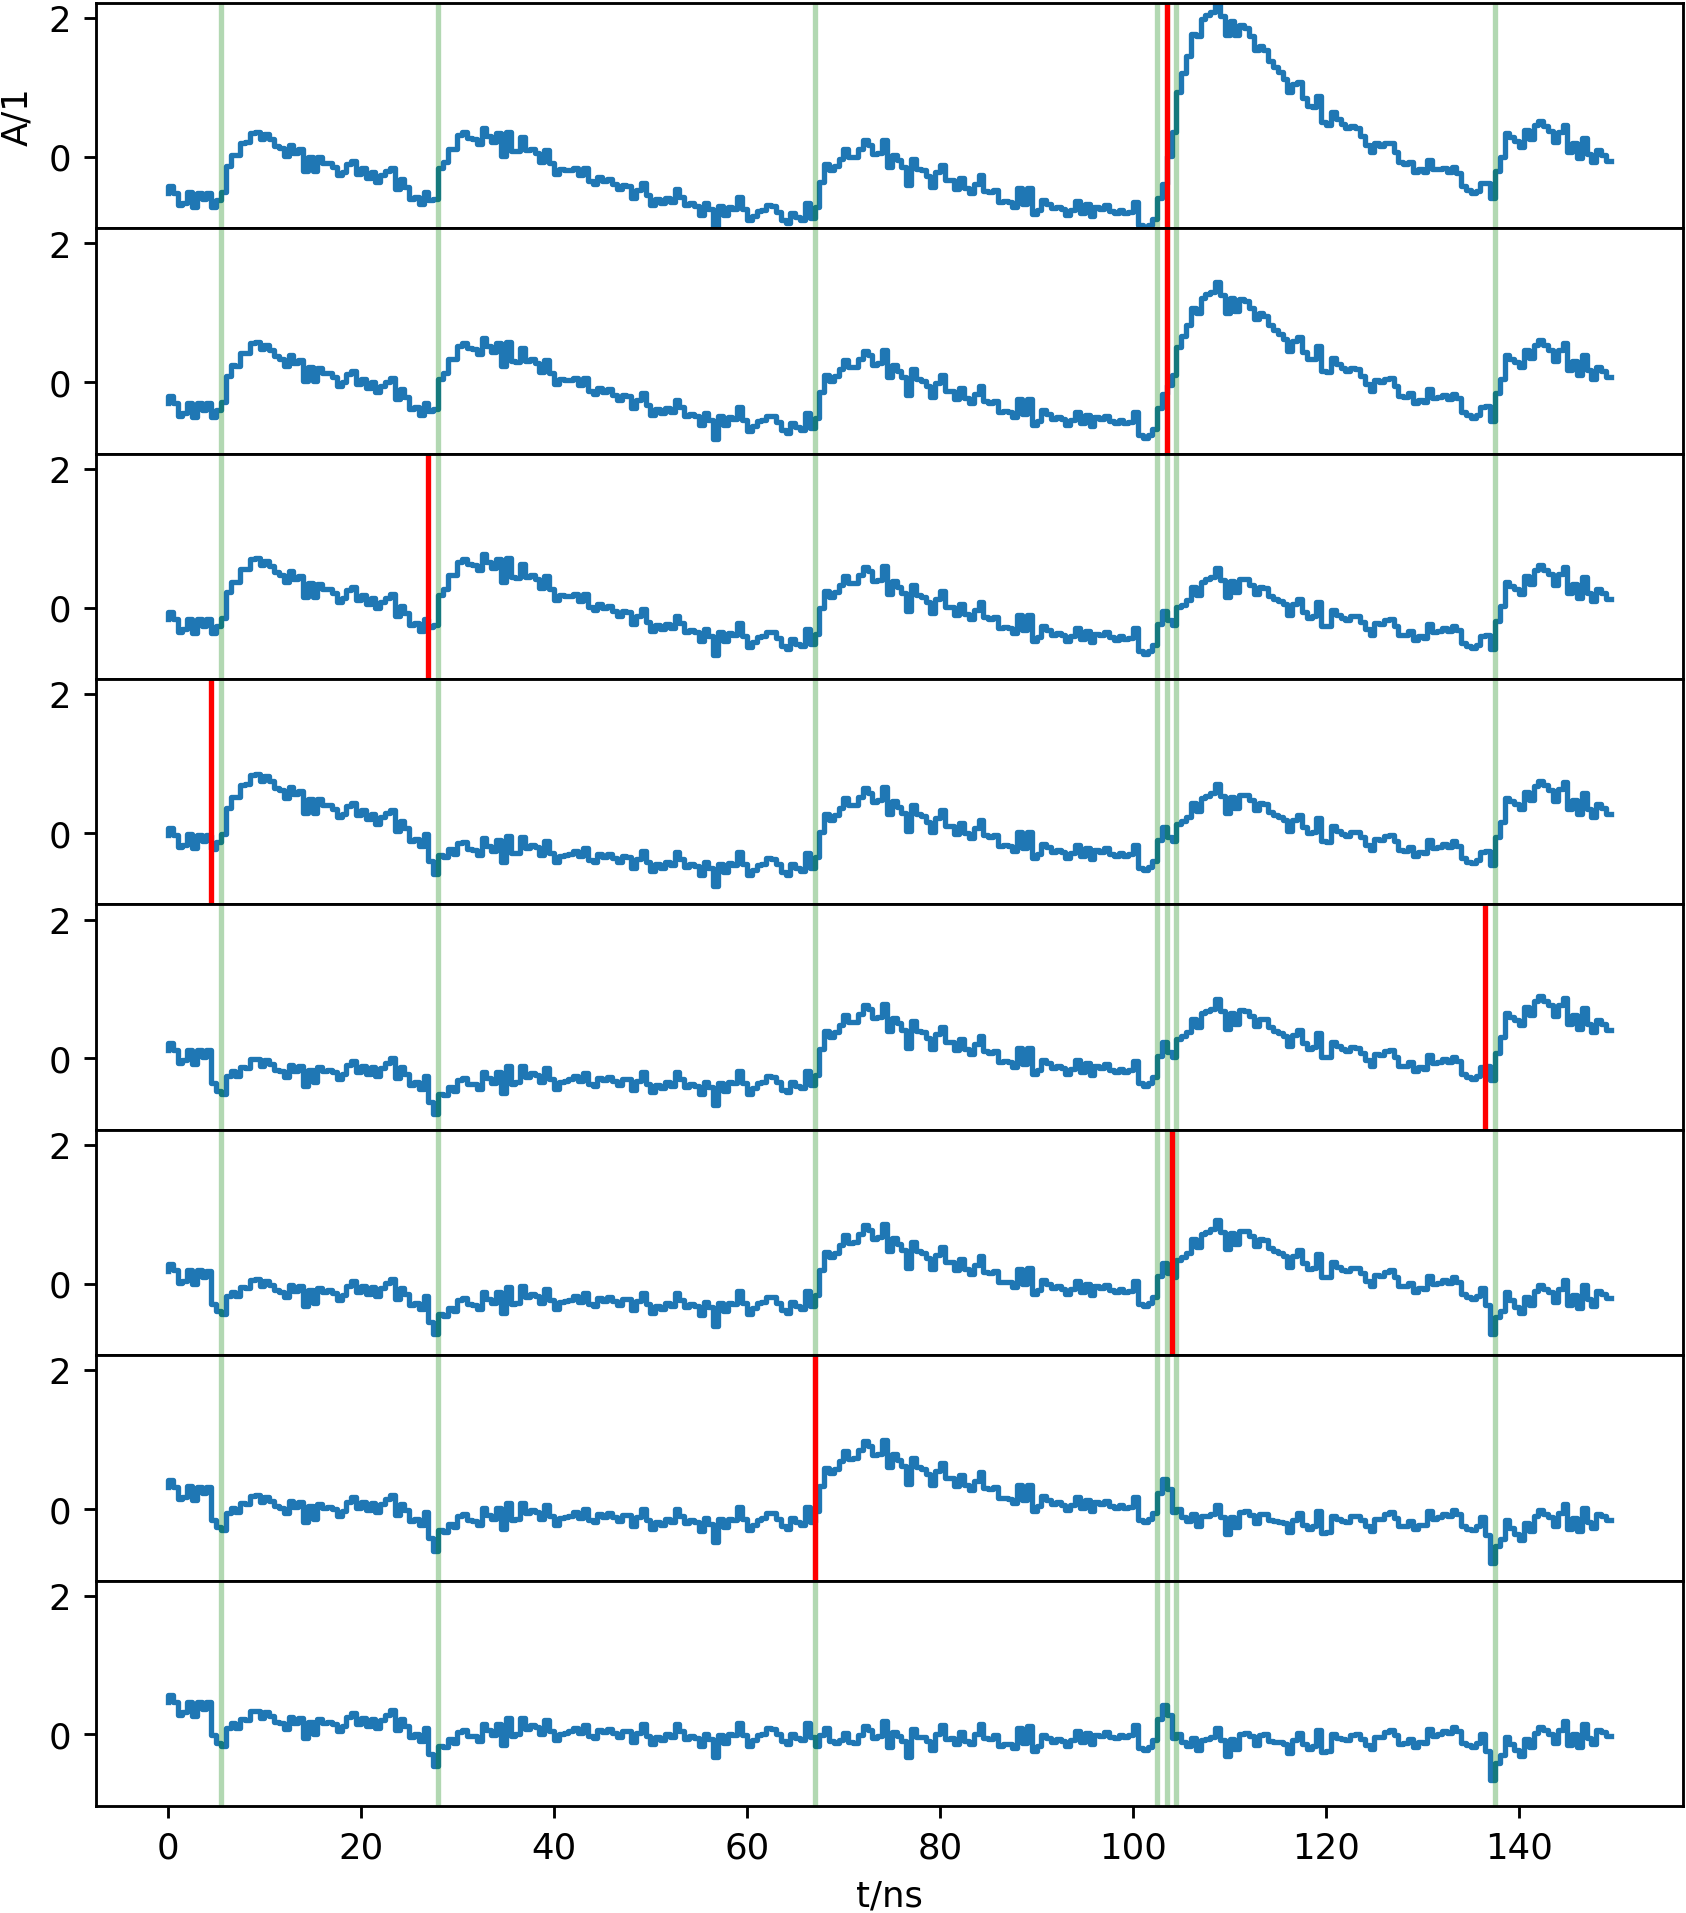
\includegraphics[width=\textwidth]{Plots/example_extraction_seed_5.png}
  \caption{Example of the photon extraction from a calibrated time series \cite{singlephs}. Shown are several steps of the iterative extraction for the time series of a single pixel. The top frame shows the full time series as returned from the calibration process. The red vertical line shows the time position of the first found photon. After subtracting the photon pulse template $T_1$, the series as shown in the frame below remains, where another photon is found at the same position (red vertical line). The extraction continues until the time series in the bottom frame remains, which is considered noise. The extracted photon arrival times represent the PhotonStream for this specific pixel.}
  \label{fig:extraction}
\end{figure}
%
\newpage
Red vertical lines
indicate the time position of a found rising edge template $T_2$. The time
series of a single pixel is correlated with $T_2$ to find the maximum of that
correlation. The response is defined as
%
\begin{equation}
  R[t] = A_\text{pixel}[t]\cdot T_2[t] \, .
\end{equation}
%
The maximum of the response is identified as the arrival time of a photon pulse.
After such a pulse has been found, the full photon pulse template $T_1$ is
subtracted. The remaining time series is then searched for further photon
pulses until only noise is left. The stopping-criterion defining the last
iteration step is reached when the maximum of the response $R[t]$ drops below
half of the maximum of the response to a single-pulse.
Every found arrival time of a photon is written to a list containing the
PhotonStream for the specific event and pixel.
